\section{Preserving raw forecasts while testing geometric utility}
\label{sec:utility-extension}

The preceding studies motivate a distinct question. Does KAHM help when
its contribution is a correction to an unchanged raw forecast, and how
does that contribution depend on training data and the raw decoder?
The extension separates these factors and tests a fixed adoption rule on
four additional archive collections. Its protocol, candidate grid, data
roster, and execution sources are frozen before its full model evaluations.
This is a prospective execution freeze, not external preregistration.
The earlier evidence and post-hoc scaling analysis remain separately
reported; no outcome from those archives is reclassified as new confirmation.

\subsection{Forecasts, controls, and selection}
\label{sec:utility-models}

The raw baseline is the inherited finite Gaussian Nystr\"om predictor with
appended linear history coordinates, column standardization, and a ridge
head. Its requested $M$ landmarks and regularization are fitted using the raw history
only. For each $g\in\{\mathrm{KAHM},\mathrm{affine},\mathrm{locality}\}$,
we fit a separate ridge head on the local-coordinate features of
Equation~\eqref{c:eq:local}, using the raw model's training residuals as
targets. The additive forecast is Equation~\eqref{eq:utility-additive}.
The correction has its own standardization and ridge penalty; it does not
change raw distances, landmarks, coefficients, or regularization, and it
introduces no additional Nystr\"om basis. Residuals are in-sample training
residuals, not cross-fitted residuals. This choice is part of the evaluated
procedure and can limit the structure left for the correction to learn.

All geometries use the same partitions, principal-direction configuration,
reference-selection rules, and fitting seeds. The geometry bank uses
three blocks of 2, 4, and 8 local models, requested rank two, at most 24
references per local model, and at most 512 fitting histories. KAHM uses
the stable Gaussian query arithmetic described in
Section~\ref{c:sec:numerical}; affine and locality controls do not fit KAHM
kernels. The concatenated raw-plus-KAHM architecture from the original
natural study is also fitted under this extension's limits. It preserves
raw information but changes the finite kernel geometry, so it is a
different complete procedure, not a restricted version of the additive
model. Raw ridge, persistence/seasonal-naive prediction, and a fixed
histogram-gradient-boosting control complete the comparison.

Validation first chooses the raw RBF penalty from
$\{0.01,1,100\}$. Holding this raw forecast fixed, each correction searches
the same three penalties and weights $\gamma\in\{0,0.25,0.5,1\}$.
There are ten distinct correction candidates: one zero correction and
nine positive-weight choices. Ties favor smaller $\gamma$, followed by
the fixed penalty order. These extra validation opportunities are part
of the additive procedure; equal landmark counts do not equalize search
size, effective function classes, or cost. The main KAHM policy uses its
selected correction only if validation MSE is at least 5\% below that of
the selected raw baseline. A second declared policy applies the same
threshold to the validation-best choice across all three geometries.
The 5\% threshold is a research sensitivity, not a test-set guarantee or
an application-derived minimum. Every policy pays for the corrections
it examines, including corrections it declines.

\subsection{Training size, raw decoder capacity, and new sources}
\label{sec:utility-design}

The synthetic factorial crosses the three inherited forecasting laws,
$N\in\{32,128\}$ independent training episodes, and
$M\in\{16,64\}$ raw RBF landmarks. Twelve fresh repetitions use seeds
9100--9111, for 144 configurations. Within a law and repetition, the 32
training episodes are a prefix of the same 128-episode collection, and
all four $N\times M$ settings share 64 validation and 128 test episodes.
Episodes retain length 72, history 12, offsets 1, 4, and 12, and 13 origins
per episode. All training origins can fit the decoder; the 512-history
limit applies only to the geometry bank. Selected forecasts use
training-only fitting, without adding validation episodes, so $N$ remains
an interpretable factor. This changes the raw predictor's capacity while
holding the correction's declared architecture fixed; it does not vary
every source of model complexity.

Synthetic MSE averages target coordinates and origins within episodes,
then episodes. The primary loss differences compare additive KAHM with
raw RBF and concatenated KAHM in each of the 12 law--$N$--$M$ cells.
All 24 contrasts use a separate family of 95\% Bonferroni paired Student
intervals over 12 complete repetitions. Their coverage relies on a
normal approximation for repetition-level differences; origins and
horizons do not increase the replication count. Affine, locality, and
practical-control means are reported without promoting their descriptive
comparisons into that primary interval family.

The archive-source evaluation uses Weather, Solar Weekly, COVID-19 Deaths,
and Car Parts with missing values from the Monash archive
\citep{Godahewa2021Monash,Godahewa2020Weather,Godahewa2020SolarWeekly,
Godahewa2020CovidDeaths,Godahewa2020CarPartsMissing}. They were absent
from the original eight-source study. Solar Weekly is an aggregation
of simulated NREL solar-production series; it is not an independent
observational solar deployment. Three training-prefix-eligible series
per collection are selected by a fixed hash ordering. Eligibility and
selection cannot use validation/test forecasting performance, and selected
series are not replaced because later evaluation is unfavorable or
unavailable. The roster is listed in Appendix~\ref{app:utility-protocol}.

Each series has chronological 60/20/20 training, validation, and test
segments. Weather and COVID use a 28-step history and all seven next
steps as direct targets; Solar Weekly and Car Parts use a six-step
history and two-step target. Fits use at most 512 available training
windows and evaluations at most 64 origins per segment, sampled evenly.
After validation selection, selected configurations are refitted on
admissible pretest windows under the same cap. Inputs use only past
observations, including already observed test values at later origins;
test targets cannot retune the fitted model. Missing values are not
interpolated. A training-only seasonal-difference MSE, with a declared
first-difference fallback, supplies the fixed scale. The two requested landmark
counts give 24 configurations. Aggregation weights capacities equally
within series, series equally within source, and the four sources equally.
These are descriptive comparisons on four selected collections, not
24 independent domains or a random sample of applications.

The main model-pipeline cost covers raw search, geometry and correction
search, validation forecasts, selected refits, final prediction, and model
serialization. Shared raw work is charged once for an additive procedure
or policy. Data preparation is recorded separately, as are model size and
prediction cost. Imports, downloads, prediction-artifact writes, and
research reporting are outside model timing. Policy costs are unions of
measured required components, not separately timed full-policy executions.
One task and one numerical-library
thread are active during timing. Wall time and available CPU components
are recorded separately. The accuracy--cost comparison therefore
describes this implementation and hardware, without claiming a minimum
necessary representation complexity. Additional fitting and audit details
appear in Appendix~\ref{app:utility-protocol}.

\subsection{Controlled utility across data and decoder budgets}
\label{sec:utility-synthetic-results}

% Generated from the audited forecasting-utility extension; no model fitting.
\begin{table}[!htbp]
\centering\small\setlength{\tabcolsep}{4pt}
\caption{New synthetic factorial: mean test MSE multiplied by $10^3$, over 12 fresh complete repetitions per cell. $N$ counts training episodes; $M$ counts raw RBF landmarks. All correction heads are ridge heads. These are cell means; simultaneous primary intervals appear in Figure~\ref{fig:utility-contrasts}.}
\label{tab:utility-synthetic}
\begin{tabular}{lrrrrrrr}
\toprule
Law & $N$ & $M$ & Raw RBF & Concat. & +KAHM & +Affine & +Locality \\
\midrule
Nonlinear AR & 32 & 16 & 4.8715 & 4.9851 & 4.7525 & 4.7586 & 4.7584 \\
Nonlinear AR & 32 & 64 & 5.0133 & 5.3388 & 5.0157 & 5.0190 & 5.0173 \\
Nonlinear AR & 128 & 16 & 4.6648 & 4.6592 & 4.5701 & 4.5805 & 4.5753 \\
Nonlinear AR & 128 & 64 & 4.4806 & 4.7006 & 4.4806 & 4.4840 & 4.4832 \\
Van der Pol & 32 & 16 & 22.0913 & 7.0925 & 15.6100 & 15.1578 & 12.8848 \\
Van der Pol & 32 & 64 & 9.2066 & 2.6518 & 8.2892 & 8.3880 & 8.0522 \\
Van der Pol & 128 & 16 & 20.5463 & 7.5690 & 14.4955 & 13.8986 & 11.5027 \\
Van der Pol & 128 & 64 & 8.4031 & 2.4087 & 7.4507 & 7.5359 & 7.0687 \\
Duffing & 32 & 16 & 7.3080 & 8.5619 & 6.6154 & 5.3215 & 5.6464 \\
Duffing & 32 & 64 & 5.3159 & 5.0348 & 5.2959 & 4.7693 & 5.0240 \\
Duffing & 128 & 16 & 6.6937 & 7.6252 & 5.8873 & 4.7225 & 4.8299 \\
Duffing & 128 & 64 & 4.3215 & 4.0529 & 4.2667 & 3.6788 & 3.8379 \\
\bottomrule
\end{tabular}
\end{table}


\begin{figure}[t]
\centering
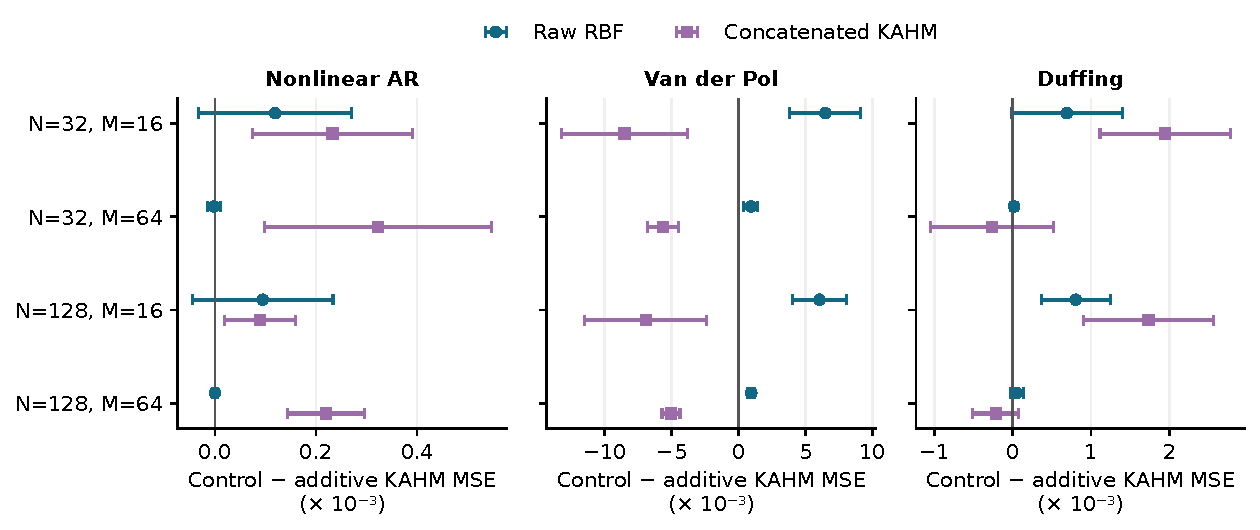
\includegraphics[width=\textwidth]{generated/utility/synthetic_contrasts.pdf}
\caption{Every primary contrast in the new factorial. Points and bars are
mean control-minus-additive-KAHM MSE and the separate 95\% Bonferroni
paired Student intervals over 12 complete repetitions. Positive values
favor additive KAHM. Each panel has its own horizontal range in the same
units; shared data within repetitions pair the $N\times M$ comparisons.
Coverage requires the stated normal approximation and does not imply a
joint claim with earlier interval families.}
\label{fig:utility-contrasts}
\end{figure}

Table~\ref{tab:utility-synthetic} reports every law--data--capacity cell,
including the simpler geometric controls. Figure~\ref{fig:utility-contrasts}
shows all primary intervals. Their lower endpoints exceed zero in
\UtilityRawPositiveContrasts{} of 12 comparisons with raw RBF and
\UtilityConcatPositiveContrasts{} of 12 comparisons with concatenated
KAHM; upper endpoints are below zero in
\UtilityRawNegativeContrasts{} and \UtilityConcatNegativeContrasts{}
comparisons, respectively. An interval spanning zero is unresolved under
this family, not evidence of equality. Complete numeric intervals and
the ridge, persistence, boosting, and fixed-policy controls are retained
in Tables~\ref{tab:utility-intervals}
and~\ref{tab:utility-synthetic-controls}.

The five resolved gains over raw RBF comprise all four Van der Pol
cells and Duffing at $N=128,M=16$. The six resolved gains over
concatenated KAHM comprise all four autoregression cells and both
16-landmark Duffing cells. Conversely, concatenated KAHM beats the
additive construction in all four Van der Pol cells. The mean gain over
raw RBF on Van der Pol is larger at 16 than at 64 landmarks for each
training size, consistent with the correction exploiting structure left
by a limited raw decoder; this is a descriptive capacity pattern, not
a tested interaction or a universal law of model size.

KAHM-specific benefit is not established by these raw-baseline contrasts.
At least one simpler additive control has lower mean error in every
Van der Pol and Duffing cell. Additive KAHM has the lowest mean among
the three additive geometries in the four autoregression cells, but
its raw-baseline intervals there remain unresolved. The fixed boosting
control has the lowest mean among all standalone methods in three
Van der Pol cells; concatenated KAHM is lowest at $N=32,M=64$.
Thus the zero-correction construction preserves a valuable forecast
option without making its ridge correction the best way to use KAHM
geometry. Neither these means nor equal raw landmark budgets establish
equal computational cost or a geometry-specific population advantage.

\subsection{Archive-source utility, selection, and cost}
\label{sec:utility-archive-results}

\paragraph{Fit feasibility is part of the result.}
All 144 synthetic configurations complete. On the archive roster, 22 of
24 configurations complete every procedure. The two capacities for Car
Parts series T1324 each have 23 training histories but only seven distinct
histories. The declared eight-group bank produces fewer nonempty groups
than requested, and the unchanged implementation raises an error rather
than silently dropping a group. Concatenated KAHM and all three additive
geometries fail on both configurations, producing eight failed model fits.
Both declared policies also fail because their required correction
candidate is unavailable. Raw ridge, raw RBF, naive, and boosting forecasts
remain available on all 24 configurations. This is a shared bank-fitting
failure; it does not isolate the KAHM kernel as its cause. No model was
refitted under a changed configuration and no series was replaced.

Consequently, the full-roster KAHM and policy mean losses are undefined.
The reporting amendment retains those failures and adds an explicitly
post-hoc matched-success diagnostic on the 22 configurations where every
procedure completes. This subset has 11 series: three each from Weather,
Solar, and COVID, and two from Car Parts. Sources retain equal weight,
with the remaining Car Parts series now sharing that source's weight.
This comparison conditions on successful fitting and changes the
prespecified roster; it is not the original full-roster estimand or a new
confirmatory transfer result. All-24 baseline outcomes remain visible.

% Generated from the audited forecasting-utility extension; no model fitting.
\begin{table}[!htbp]
\centering\small\setlength{\tabcolsep}{4pt}
\caption{New archive-source coverage and losses. Full-roster scaled MSE uses all 24 configurations and is undefined (dash) for procedures with failed fits. Matched loss and wall seconds use only the post-hoc 22-configuration common-support diagnostic (11 series, including two Car Parts series), with equal source weights. Pipeline costs include all required searches, validation, selected refit, prediction, and serialization. Policy costs are unions of measured required components, including rejected corrections; they are not separately timed full policy executions. Conditioning on success does not complete the prespecified full-roster evaluation.}
\label{tab:utility-archive}
\begin{tabular}{lrrrr}
\toprule
Procedure & Outputs & Full-roster MSE & Matched MSE & Matched seconds \\
\midrule
Raw ridge & 24/24 & 1.2848 & 0.8466 & 0.0015 \\
Raw RBF & 24/24 & 9.6633 & 9.1730 & 0.0037 \\
Concatenated KAHM & 22/24 & \textemdash & 1.2111 & 0.0691 \\
Additive KAHM & 22/24 & \textemdash & 9.1443 & 0.0498 \\
Additive affine & 22/24 & \textemdash & 9.3312 & 0.0369 \\
Additive locality & 22/24 & \textemdash & 9.5624 & 0.0379 \\
Persistence / seasonal naive & 24/24 & 1.5720 & 1.2062 & 0.0012 \\
Histogram gradient boosting & 24/24 & 10.7552 & 10.3174 & 0.6380 \\
KAHM 5\% rule & 22/24 & \textemdash & 9.2460 & 0.0467 \\
All-geometry 5\% rule & 22/24 & \textemdash & 9.2624 & 0.0869 \\
\bottomrule
\end{tabular}
\end{table}


Table~\ref{tab:utility-archive} reports coverage, full-roster losses where
defined, and the separate matched-success diagnostic. Source-specific
losses, leave-one-source-out summaries, actual decoder dimensions, and
all selected mixing weights appear in Appendix~\ref{app:utility-results}.
Among the 22 completed archive comparisons, the KAHM policy adopts a
correction on \UtilityKAHMAdoptions{} configurations and the all-geometry
policy on \UtilityGeometryAdoptions{}. Their decisions use only validation
outcomes. Their matched-success costs include searching corrections even
when the selected test forecast is the raw baseline, but do not redefine
the two failed policy evaluations as successful raw decisions.

On the matched-success diagnostic, raw RBF, concatenated KAHM, and
additive KAHM have scaled MSEs \UtilityRawLoss{}, \UtilityConcatLoss{},
and \UtilityKAHMLoss{}, respectively. The additive improvement over
raw RBF is only \UtilityKAHMGainPercent\% at
\UtilityKAHMCostRatio{} times its measured model-pipeline wall cost.
Raw ridge is both more accurate, at \UtilityRidgeLoss{}, and cheaper,
at \UtilityRidgeCostRatio{} times the raw RBF cost. Concatenated KAHM
substantially improves this weak raw RBF comparator on the diagnostic
subset, but remains worse than raw ridge and has undefined full-roster
loss because of the two failed fits. This is why utility must be judged
against credible simpler alternatives as well as a matched architectural
baseline.

The KAHM 5\% rule has matched-success loss \UtilityPolicyLoss{} at
\UtilityPolicyCostRatio{} times raw RBF's model-pipeline cost; the
all-geometry rule has loss \UtilityGeometryPolicyLoss{} at
\UtilityGeometryPolicyCostRatio{} times its cost. Neither improves
aggregate error on that subset. Positive validation gains therefore do
not establish beneficial test corrections after the pretest refit.

The source detail explains the small additive KAHM aggregate change:
COVID is its only improving source mean, Solar is unchanged, and Weather
and Car Parts worsen. Excluding COVID reverses the aggregate direction
(Table~\ref{tab:utility-leave-one}); this is sensitivity of the same
diagnostic, not additional evidence. The saved-prediction decomposition
likewise has KAHM alignment exceeding correction energy only on COVID,
zero correction on Solar, and negative net gains on the other two sources
(Table~\ref{tab:utility-residual}). The identity verifies how the realized
corrections change squared error without estimating the oracle residual
structure or rescuing the incomplete full-roster evaluation.
